\documentclass[11pt,a4paper]{report}

% Institutional and submission metadata (CMP6230 coursework brief summary)
\newcommand{\UniName}{Birmingham City University}
\newcommand{\StudentName}{Nabin Oli}
\newcommand{\StudentID}{23189629}
\newcommand{\DegreeName}{BSc (Hons) Computer and Data Science}

\newcommand{\ModuleCode}{CMP6230}
\newcommand{\TaskName}{Coursework Task 1}
\newcommand{\ReportTitle}{Data Analytics Pipeline Planning and Design}

\title{\ReportTitle}
\author{\StudentName}
\date{\today}

% Typography and layout
\usepackage[T1]{fontenc}
\usepackage[utf8]{inputenc}
\usepackage[british]{babel}

\usepackage[a4paper,margin=25mm]{geometry}
\usepackage{microtype}
\usepackage{setspace}
\onehalfspacing

\usepackage{csquotes}
\usepackage{amsmath,amssymb}

\usepackage{graphicx}
\graphicspath{{figures/}{figures/logos/}{figures/appendix/}}

\usepackage{tikz}
\usetikzlibrary{positioning,shapes.geometric,arrows.meta,calc,fit,backgrounds,
                decorations.pathreplacing,shadows.blur}
\usepackage{fontawesome5}

\usepackage{simpleicons}

% Publication-grade TikZ design system for MLOps diagrams (CMP6230 report).
% Oxford Blue + Burgundy palette; loaded via % Publication-grade TikZ design system for MLOps diagrams (CMP6230 report).
% Oxford Blue + Burgundy palette; loaded via \input{tikz/mlops-styles}.

\newdimen\mlopsStageTextWd
\mlopsStageTextWd=27mm

% --- Palette ---------------------------------------------------------------
\definecolor{oxfordPrimary}{RGB}{11,37,69}
\definecolor{oxfordPrimarySoft}{RGB}{36,67,108}
\definecolor{accentBurgundy}{RGB}{140,47,57}
\definecolor{dataplaneTint}{RGB}{238,242,248}
\definecolor{controlplaneTint}{RGB}{244,241,236}
\definecolor{cardFill}{RGB}{255,255,255}
\definecolor{cardSubtle}{RGB}{250,250,248}
\definecolor{inkBody}{RGB}{40,46,58}
\definecolor{inkMuted}{RGB}{95,105,120}

% Back-compat aliases (older diagrams / drafts)
\colorlet{mlopsDataplaneBg}{dataplaneTint}
\colorlet{mlopsControlBg}{controlplaneTint}
\colorlet{mlopsStageFill}{cardFill}
\colorlet{mlopsStageBorder}{oxfordPrimary}
\colorlet{mlopsSubstageFill}{cardSubtle}
\colorlet{mlopsAccent}{accentBurgundy}

\tikzset{
  % Outer shell for pipeline stages (used by \mlopsStage)
  mlops stage shell/.style={
    rounded corners=5pt,
    draw=oxfordPrimary,
    line width=0.65pt,
    fill=cardFill,
    align=center,
    inner sep=8pt,
    minimum width=31mm,
    text width=31mm,
    font=\scriptsize,
    text=inkBody,
  },
  mlops stage badge/.style={
    circle,
    fill=white,
    text=oxfordPrimary,
    font=\fontsize{7}{7}\selectfont\sffamily\bfseries,
    inner sep=0pt,
    minimum size=5mm,
    draw=white,
    line width=0.35pt,
  },
  mlops substage/.style={
    rounded corners=4pt,
    draw=oxfordPrimarySoft,
    line width=0.55pt,
    fill=cardSubtle,
    align=center,
    inner sep=5pt,
    font=\footnotesize,
    text=inkBody,
    text width=31mm,
  },
  mlops dataarrow/.style={
    -{Stealth[length=2.5mm,width=1.75mm]},
    line width=0.7pt,
    draw=oxfordPrimary,
    rounded corners=1.5pt,
    shorten >=1.8pt,
    shorten <=1.8pt,
  },
  mlops feedbackarrow/.style={
    -{Stealth[length=2.2mm,width=1.55mm]},
    line width=0.65pt,
    dashed,
    draw=accentBurgundy,
    rounded corners=2pt,
    shorten >=1.5pt,
    shorten <=1.5pt,
  },
  mlops feedback label/.style={
    fill=white,
    draw=accentBurgundy!58,
    rounded corners=2pt,
    inner sep=2.5pt,
    font=\tiny\sffamily\bfseries,
    text=accentBurgundy,
  },
  mlops swimlane fill/.style={
    rounded corners=7pt,
    inner sep=11pt,
  },
  mlops swimlane title pill/.style={
    fill=white,
    draw=oxfordPrimarySoft!55,
    rounded corners=2.5pt,
    inner sep=3pt,
    font=\footnotesize\scshape,
    text=oxfordPrimary,
  },
  mlops persona/.style={
    circle,
    draw=oxfordPrimarySoft,
    line width=0.55pt,
    fill=white,
    minimum size=7.5mm,
    inner sep=0pt,
    font=\scriptsize,
    text=inkBody,
  },
  mlops persona link/.style={
    draw=oxfordPrimarySoft!70,
    dotted,
    line width=0.45pt,
    -,
    shorten >=1pt,
    shorten <=1pt,
  },
  mlops ctrl link/.style={
    draw=oxfordPrimarySoft!35,
    dotted,
    line width=0.4pt,
    -,
    shorten >=1.5pt,
    shorten <=1.5pt,
  },
  mlops legend container/.style={
    rounded corners=4pt,
    draw=oxfordPrimarySoft!45,
    fill=white,
    inner sep=6pt,
    font=\footnotesize\sffamily,
    text=inkBody,
  },
}

% Stage card: \mlopsStage[<node keys>]{name}{number}{icons}{title}{body}
\newcommand{\mlopsStage}[6][]{% #1 optional positioning/style keys
  \node[mlops stage shell, #1] (#2) {%
    \begin{minipage}{\mlopsStageTextWd}%
      \centering
      \setlength{\fboxsep}{5pt}%
      \colorbox{oxfordPrimary}{%
        \parbox[c][7.5mm][c]{\dimexpr\linewidth-10pt}{%
          \makebox[\dimexpr\linewidth-10pt][c]{%
            \raisebox{-0.6pt}{\tikz[baseline=-1mm]{\node[mlops stage badge]{#3};}}%
            \kern4pt%
            \textbf{\textcolor{white}{\small #5}}%
          }%
        }%
      }\par\vspace{4pt}%
      {\centering\mbox{#4}\par}%
      \vspace{4pt}%
      {\centering\footnotesize\color{inkMuted}#6\par}%
    \end{minipage}%
  };%
}

% Two-tool icon row for stage bodies (PNG / Simple Icons fallback align uniformly).
\newcommand{\mlopsToolPair}[2]{\raisebox{-1pt}{\hbox{#1\kern1.5pt#2}}}
.

\newdimen\mlopsStageTextWd
\mlopsStageTextWd=27mm

% --- Palette ---------------------------------------------------------------
\definecolor{oxfordPrimary}{RGB}{11,37,69}
\definecolor{oxfordPrimarySoft}{RGB}{36,67,108}
\definecolor{accentBurgundy}{RGB}{140,47,57}
\definecolor{dataplaneTint}{RGB}{238,242,248}
\definecolor{controlplaneTint}{RGB}{244,241,236}
\definecolor{cardFill}{RGB}{255,255,255}
\definecolor{cardSubtle}{RGB}{250,250,248}
\definecolor{inkBody}{RGB}{40,46,58}
\definecolor{inkMuted}{RGB}{95,105,120}

% Back-compat aliases (older diagrams / drafts)
\colorlet{mlopsDataplaneBg}{dataplaneTint}
\colorlet{mlopsControlBg}{controlplaneTint}
\colorlet{mlopsStageFill}{cardFill}
\colorlet{mlopsStageBorder}{oxfordPrimary}
\colorlet{mlopsSubstageFill}{cardSubtle}
\colorlet{mlopsAccent}{accentBurgundy}

\tikzset{
  % Outer shell for pipeline stages (used by \mlopsStage)
  mlops stage shell/.style={
    rounded corners=5pt,
    draw=oxfordPrimary,
    line width=0.65pt,
    fill=cardFill,
    align=center,
    inner sep=8pt,
    minimum width=31mm,
    text width=31mm,
    font=\scriptsize,
    text=inkBody,
  },
  mlops stage badge/.style={
    circle,
    fill=white,
    text=oxfordPrimary,
    font=\fontsize{7}{7}\selectfont\sffamily\bfseries,
    inner sep=0pt,
    minimum size=5mm,
    draw=white,
    line width=0.35pt,
  },
  mlops substage/.style={
    rounded corners=4pt,
    draw=oxfordPrimarySoft,
    line width=0.55pt,
    fill=cardSubtle,
    align=center,
    inner sep=5pt,
    font=\footnotesize,
    text=inkBody,
    text width=31mm,
  },
  mlops dataarrow/.style={
    -{Stealth[length=2.5mm,width=1.75mm]},
    line width=0.7pt,
    draw=oxfordPrimary,
    rounded corners=1.5pt,
    shorten >=1.8pt,
    shorten <=1.8pt,
  },
  mlops feedbackarrow/.style={
    -{Stealth[length=2.2mm,width=1.55mm]},
    line width=0.65pt,
    dashed,
    draw=accentBurgundy,
    rounded corners=2pt,
    shorten >=1.5pt,
    shorten <=1.5pt,
  },
  mlops feedback label/.style={
    fill=white,
    draw=accentBurgundy!58,
    rounded corners=2pt,
    inner sep=2.5pt,
    font=\tiny\sffamily\bfseries,
    text=accentBurgundy,
  },
  mlops swimlane fill/.style={
    rounded corners=7pt,
    inner sep=11pt,
  },
  mlops swimlane title pill/.style={
    fill=white,
    draw=oxfordPrimarySoft!55,
    rounded corners=2.5pt,
    inner sep=3pt,
    font=\footnotesize\scshape,
    text=oxfordPrimary,
  },
  mlops persona/.style={
    circle,
    draw=oxfordPrimarySoft,
    line width=0.55pt,
    fill=white,
    minimum size=7.5mm,
    inner sep=0pt,
    font=\scriptsize,
    text=inkBody,
  },
  mlops persona link/.style={
    draw=oxfordPrimarySoft!70,
    dotted,
    line width=0.45pt,
    -,
    shorten >=1pt,
    shorten <=1pt,
  },
  mlops ctrl link/.style={
    draw=oxfordPrimarySoft!35,
    dotted,
    line width=0.4pt,
    -,
    shorten >=1.5pt,
    shorten <=1.5pt,
  },
  mlops legend container/.style={
    rounded corners=4pt,
    draw=oxfordPrimarySoft!45,
    fill=white,
    inner sep=6pt,
    font=\footnotesize\sffamily,
    text=inkBody,
  },
}

% Stage card: \mlopsStage[<node keys>]{name}{number}{icons}{title}{body}
\newcommand{\mlopsStage}[6][]{% #1 optional positioning/style keys
  \node[mlops stage shell, #1] (#2) {%
    \begin{minipage}{\mlopsStageTextWd}%
      \centering
      \setlength{\fboxsep}{5pt}%
      \colorbox{oxfordPrimary}{%
        \parbox[c][7.5mm][c]{\dimexpr\linewidth-10pt}{%
          \makebox[\dimexpr\linewidth-10pt][c]{%
            \raisebox{-0.6pt}{\tikz[baseline=-1mm]{\node[mlops stage badge]{#3};}}%
            \kern4pt%
            \textbf{\textcolor{white}{\small #5}}%
          }%
        }%
      }\par\vspace{4pt}%
      {\centering\mbox{#4}\par}%
      \vspace{4pt}%
      {\centering\footnotesize\color{inkMuted}#6\par}%
    \end{minipage}%
  };%
}

% Two-tool icon row for stage bodies (PNG / Simple Icons fallback align uniformly).
\newcommand{\mlopsToolPair}[2]{\raisebox{-1pt}{\hbox{#1\kern1.5pt#2}}}

% Hybrid logos: prefer files under figures/logos/ (\graphicspath),
% else Simple Icons font glyphs. Loaded after graphicx + simpleicons.

\newcommand{\MLOpsLogo}[4]{%
  \IfFileExists{#1.png}{%
    \includegraphics[height=#4]{#1.png}%
  }{%
    \IfFileExists{#1.pdf}{%
      \includegraphics[height=#4]{#1.pdf}%
    }{%
      \resizebox{!}{#4}{\mbox{\simpleicon{#2}}}%
    }%
  }%
}

\newcommand{\AirflowLogo}[1][9mm]{\MLOpsLogo{airflow}{apacheairflow}{Airflow}{#1}}
\newcommand{\KafkaLogo}[1][9mm]{\MLOpsLogo{kafka}{apachekafka}{Kafka}{#1}}
\newcommand{\SparkLogo}[1][9mm]{\MLOpsLogo{spark}{apachespark}{Spark}{#1}}
\newcommand{\MLflowLogo}[1][9mm]{\MLOpsLogo{mlflow}{mlflow}{MLflow}{#1}}
\newcommand{\DockerLogo}[1][9mm]{\MLOpsLogo{docker}{docker}{Docker}{#1}}
\newcommand{\KubernetesLogo}[1][9mm]{\MLOpsLogo{kubernetes}{kubernetes}{Kubernetes}{#1}}
\newcommand{\PrometheusLogo}[1][9mm]{\MLOpsLogo{prometheus}{prometheus}{Prometheus}{#1}}
\newcommand{\GrafanaLogo}[1][9mm]{\MLOpsLogo{grafana}{grafana}{Grafana}{#1}}
\newcommand{\DbtLogo}[1][9mm]{\MLOpsLogo{dbt}{dbt}{dbt}{#1}}
\newcommand{\JupyterLogo}[1][9mm]{\MLOpsLogo{jupyter}{jupyter}{Jupyter}{#1}}


\usepackage{enumitem}
\usepackage{booktabs,tabularx,longtable}
\usepackage{caption}
\captionsetup{font=small,labelfont=bf}

\usepackage{subcaption}

\usepackage{listings}
\lstdefinelanguage{PGN}{
  sensitive=false,
  alsoletter={-:},
  morestring=[b]",
}

\lstset{
  basicstyle=\ttfamily\footnotesize,
  breaklines=true,
  breakatwhitespace=true,
  columns=fullflexible,
  frame=single,
  framerule=0.4pt,
  xleftmargin=0.65em,
  framexleftmargin=0.55em,
}

% References (hyperref must precede cleveref)
\usepackage[hidelinks,unicode]{hyperref}
\hypersetup{
  pdfauthor={\StudentName},
  pdftitle={\ReportTitle},
}
\usepackage{cleveref}

\usepackage[
  backend=biber,
  style=numeric-comp,
  sorting=none,
  maxbibnames=99,
]{biblatex}
\addbibresource{references.bib}

\setcounter{secnumdepth}{3}
\setcounter{tocdepth}{2}


\begin{document}

% Avoid duplicate Hyperref anchors on Title Page / first body page (pdfLaTeX)
\hypersetup{pageanchor=false}
\begin{titlepage}
  \centering

  {\large \UniName\par}

  \vspace*{3cm}

  {\LARGE\bfseries \ReportTitle\par}

  \vspace{0.75cm}

  {\large \ModuleCode\quad\textemdash\quad\TaskName\par}

  \vfill

  \begin{tabular}{@{}rl@{}}
    \textit{Student:}           & \StudentName \\[0.35em]
    \textit{Student ID:}        & \StudentID \\[0.35em]
    \textit{Programme of study:} & \DegreeName \\
  \end{tabular}

  \vspace{2.5cm}

  {\large \today\par}
\end{titlepage}
\hypersetup{pageanchor=true}
\cleardoublepage

\chapter*{Abstract}
\phantomsection
\addcontentsline{toc}{chapter}{Abstract}

This log report outlines the planning and design of a data management and analytics strategy for supervised machine learning within a chosen problem domain.
It traces how candidate datasets are justified, how an end-to-end analytics pipeline satisfies reporting and modelling consumers, how data will be structured after ingestion with explicit trade-offs, and how these plans iterate as understanding improves.

\tableofcontents
\clearpage

\listoffigures
\listoftables
\clearpage

\chapter{Candidate source datasets}
\label{ch:candidate-datasets}

\begin{figure}[htbp]
  \centering
  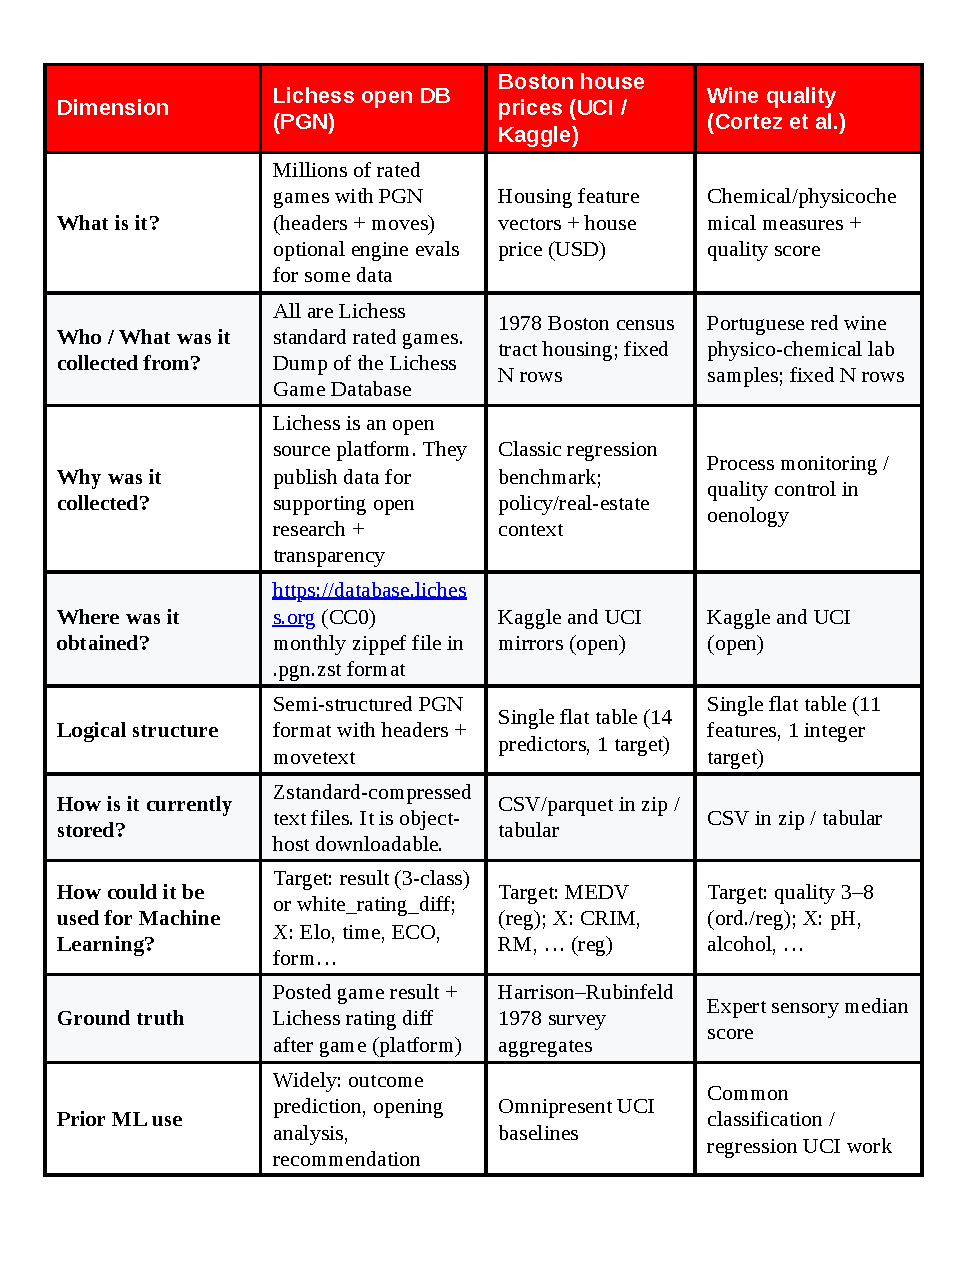
\includegraphics[width=\linewidth,keepaspectratio]{step1.pdf}
  \caption{Candidate dataset comparison across provenance, structure, storage, and supervised-learning affordances.}
  \label{fig:step1-candidate-matrix}
\end{figure}

Competitive platforms and public benchmarks offer contrasting source-data profiles for supervised
learning. This chapter evaluates three candidates transactional game telemetry, tabular chemistry
data, and census-derived housing attributes---and selects one for downstream pipeline design.
\Cref{fig:step1-candidate-matrix} summarises three candidates across provenance, structure, storage, and supervised-learning affordances.

\section[Dataset one]{Candidate dataset \textnumero\,1}
\label{sec:dataset-one}

\textbf{Lichess} ships monthly rated \texttt{.pgn.zst} archives (\url{https://database.lichess.org/}) with outcomes, clocks, ratings, openings, and SAN movelists under a \textsc{cc}0 licence~\cite{lichess_open_database}; see~\cref{app:lichess-open-database} for inventory.
Headers plus ordered moves form the logical model; physically the corpus is compressed text shards, not ready-made tables.
Supervised targets include game outcome (\texttt{[Result]}) and rating-based signals from pre-game headers (\cref{fig:lichess-pgn-sample}).

\begin{table}[h]
\centering
\caption{Lichess Chess Games (2013–present)}
\begin{tabular}{|p{0.25\textwidth}|p{0.65\textwidth}|}
\hline
\textbf{Field} & \textbf{Description} \\
\hline
Source & \url{https://database.lichess.org/} \\
\hline
Format & .pgn.zst (compressed Portable Game Notation using Zstandard) \\
\hline
Size & Jan 2013: 17.8 MB compressed. \\
      & Total: 2.49 TB, 7,863,012,346 games. \\
\hline
Features & Event, Site, Date, Round, White, Black, Result, UTCDate, UTCTime, \\
          & WhiteElo, BlackElo, WhiteRatingDiff, BlackRatingDiff, WhiteTitle, \\
          & ECO, Opening, TimeControl, Termination, \%eval, \%clk, \ldots \\
\hline
Target Variable & Game Outcome (win/loss/draw) \\
\hline
Time Period & January 2013 to present (monthly releases) \\
\hline
\end{tabular}
\end{table}

\section[Dataset two]{Candidate dataset \textnumero\,2}
\label{sec:dataset-two}

\textbf{Wine Quality}~\cite{Cortez2009wine,UCIWineQuality} is a static CSV of physicochemical assays with ordinal quality scores collected from Portuguese wine samples.
Flat relational structure and simple ingestion suit tabular baselines, but the corpus is small, stale, and lacks the temporal refresh needed for operational MLOps practice (\cref{fig:uci-wine-schema}).

\begin{table}[h]
\centering
\caption{Wine Quality (UCI)}
\begin{tabular}{|p{0.25\textwidth}|p{0.65\textwidth}|}
\hline
\textbf{Field} & \textbf{Description} \\
\hline
Source & \url{https://archive.ics.uci.edu/dataset/186/wine+quality} \\
\hline
Format & CSV \\
\hline
Size & 89 KB \\
\hline
Features & fixed\_acidity, volatile\_acidity, citric\_acid, residual\_sugar, \\
          & chlorides, free\_sulfur\_dioxide, total\_sulfur\_dioxide, density, \\
          & pH, sulphates, alcohol \\
\hline
Target Variable & quality (score) \\
\hline
Time Period & 2009 \\
\hline
\end{tabular}
\end{table}



\section[Dataset three]{Candidate dataset \textnumero\,3}
\label{sec:dataset-three}

\textbf{Boston housing}~\cite{HarrisonRubinfeld1978,UCIBostonHousing} comprises census and environmental attributes for Boston-area tracts with median home value (\texttt{MEDV}) as a continuous regression target.
The fixed flat-file schema suits classic tabular baselines rather than transactional chess telemetry and offers limited scale for ingestion, validation, and feature-store design (\cref{fig:boston-housing-sample}).

\begin{table}[h]
\centering
\caption{Boston Housing}
\begin{tabular}{|p{0.25\textwidth}|p{0.65\textwidth}|}
\hline
\textbf{Field} & \textbf{Description} \\
\hline
Source & \url{https://lib.stat.cmu.edu/datasets/boston} \\
\hline
Format & Fixed‑width formatted text file \\
\hline
Size & 506 rows × 14 columns, ~27 KB (compressed ~7 KB) \\
\hline
Features & CRIM, ZN, INDUS, CHAS, NOX, RM, AGE, DIS, RAD, TAX, \\
          & PTRATIO, B, LSTAT \\
\hline
Target Variable & MEDV (median value of owner‑occupied homes in \$1000’s) \\
\hline
Time Period & 1970s \\
\hline
\end{tabular}
\end{table}

\section{Chosen dataset and justification}
\label{sec:chosen-dataset}

We select the Lichess open database for MLOps development due to its sheer volume, scale, embedded labels, \textsc{cc}0 licensing, and monthly refresh.  Lichess dataset clearly outweighes the simpler study purpose datasets like Wine Quality and Boston housing baselines (\cref{sec:dataset-two,sec:dataset-three,fig:step1-candidate-matrix}). Additionally, Lichess Data is produced from a live platform with a large user base, so it has a real-world provenance and operational profile that suits and provides ample direction for learning opportunity in MLOps pipeline design and Data Management. 

% Following are table summarising the operational profile of the Lichess dataset which further supports this selection choice (\cref{tab:lichess-operational-profile,tab:lichess-ml-features}).


% \begin{table}[htbp]
%   \centering
%   \caption{Operational profile of the selected Lichess corpus.}
%   \label{tab:lichess-operational-profile}
%   \small
%   \setlength{\tabcolsep}{4pt}
%   \renewcommand{\arraystretch}{1.15}
%   \begin{tabular}{@{}>{\raggedright\arraybackslash}p{0.21\linewidth}
%                   >{\raggedright\arraybackslash}p{0.73\linewidth}@{}}
%     \toprule
%     Dimension & Assessment\\
%     \midrule
%     Volume and velocity &
%       Approximately \(7.68\times10^{9}\) rated games in \(\sim\)2.43\,TB of Zstandard-compressed PGN (\cref{app:lichess-open-database}).
%       Non-cumulative monthly dumps add on the order of \(5\times10^{7}\)--\(10^{8}\) games per month.\\
%     Schema complexity &
%       No fixed relational schema
%       Movetext is encoded in SAN, requiring parse or tokenisation pipelines.
%       Field inventories evolve gradually---newer months introduce headers such as \texttt{[Accuracy]} or \texttt{[Termination]} absent from early releases.\\
%     Data quality and sparsity &
%       Mix of elite (\(\geq 2500\) Elo) and casual pairings; optional tags may be absent (\texttt{[Opening]} unset for off-book positions).
%       Outcome priors are tempo-dependent: draws account for \(<2\%\) of bullet (\texttt{1+0}) games but approach \(10\)--\(15\%\) under classical controls.
%       Rating-delta targets are noisy when provisional ratings apply to new accounts.\\
%     Temporal and causal structure &
%       UTC timestamps support chronological splits and back-testing; monthly partitions suit incremental ingestion.
%       Player-level correlation violates independence for rating-change targets---splits should respect time or player identifiers, not naive random shuffling.\\
%     Operational limitation &
%       Bulk exports are post hoc monthly artefacts, not a live stream.
%       Near-real-time inference would require a complementary WebSocket feed in addition to the open-database cadence.\\
%     \bottomrule
%   \end{tabular}
% \end{table}

\subsection{Supervised modelling}
\label{sec:supervised-modelling}

The primary supervised task is \emph{pre-game outcome prediction}: given features available before the first move (ratings, time control, variant), estimate whether White wins, Black wins, or the game is drawn, a three-class classification problem with ground truth in \texttt{[Result]} (\texttt{1-0}, \texttt{0-1}, \texttt{1/2-1/2}).
% \Cref{tab:lichess-ml-features} maps labels, baseline predictors, PGN sources, and modelling caveats.

% \begin{table}[htbp]
%   \centering
%   \caption{Machine learning features and labels derivable from the Lichess dataset.}
%   \label{tab:lichess-ml-features}
%   \footnotesize
%   \setlength{\tabcolsep}{3.5pt}
%   \renewcommand{\arraystretch}{1.12}
%   \begin{tabular}{@{}>{\raggedright\arraybackslash}p{0.13\linewidth}
%                   >{\raggedright\arraybackslash}p{0.27\linewidth}
%                   >{\raggedright\arraybackslash}p{0.28\linewidth}
%                   >{\raggedright\arraybackslash}p{0.26\linewidth}@{}}
%     \toprule
%     Role & ML construct & Principal sources & Ground truth / caveats\\
%     \midrule
%     Label &
%       Game outcome (White win\,/\,draw\,/\,Black win). &
%       \texttt{[Result]} (\texttt{1-0}, \texttt{1/2-1/2}, \texttt{0-1}). &
%       Terminal result on record is the supervised ground truth; validate parsing across shards; expect tempo-dependent class skew.\\
%     Feature &
%       Relative strength / pairing imbalance. &
%       \texttt{[WhiteElo]}, \texttt{[BlackElo]}, derived rating gap (and titles if headers include them). &
%       Ratings proxy skill but drift over months; handle missing or placeholder (\texttt{?}) values for unrated or anonymous games.\\
%     Feature &
%       Clock format / tempo regime. &
%       \texttt{[TimeControl]}; chess variant headers when analysing non-standard rulesets. &
%       Strong behavioural prior; bucket bullet\,/\,blitz\,/\,rapid\,/\,classical during preprocessing for stability.\\
%     Feature &
%       Opening / early trajectory signal. &
%       First \(N\) half-moves from the SAN movelist; optional \texttt{[ECO]} when present in headers. &
%       Very high cardinality; employ hashing, embeddings, or clustering; beware transpositions if enriching from external opening tables.\\
%     Feature &
%       Length / pace proxies. &
%       Ply count from SAN tokens; optional \texttt{\%clk} timestamps alongside \texttt{[UTCDate]} / \texttt{[UTCTime]} comments when exported. &
%       Signals complexity or time trouble; clock commentary is shard-dependent---treat as optional enrichment, not assumed globally.\\
%     Feature &
%       Termination channel. &
%       \texttt{[Termination]} when present (mate, resignation, timeout, etc.). &
%       Post-game metadata; exclude from pre-game predictors or treat as diagnostic only---often correlated with outcome.\\
%     Feature &
%       Position-derived telemetry (advanced). &
%       Parsed positions (material balance, mobility); optional engine evaluations via offline joins. &
%       Highest fidelity but requires full SAN parsing or auxiliary computation; heavier engineering than header-only baselines.\\
%     \bottomrule
%   \end{tabular}
% \end{table}

\chapter{Pipeline planning and design}
\label{ch:pipeline-planning}

Analysts need notebooks and ad hoc SQL; ML engineers need scheduled training with promotion gates.
We separate stable contracts (configs, artefacts, lineage) from replaceable infrastructure (orchestrator, object store, registry).

\section{Consumer obligations and guiding principles}
\label{sec:consumers-principles}

Non-functionals: recover partial runs, audit lineage, alert on ingestion or deploy failure.
Stack shape: Airflow-class DAGs, S3-compatible storage, MLflow-style experiment tracking.

\section{Stage coverage: ingestion through monitoring}
\label{sec:pipeline-stages-global}

\begin{figure}[htbp]
  \centering
  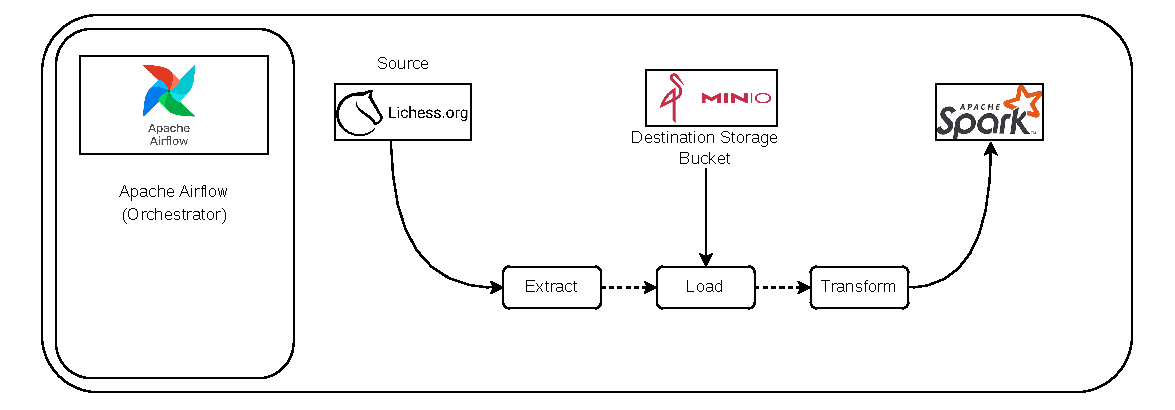
\includegraphics[width=\linewidth,height=0.55\textheight,keepaspectratio]{elt.pdf}
  \caption{ELT pattern with object storage.}
  \label{fig:etl-flow}
\end{figure}

\begin{figure}[htbp]
  \centering
  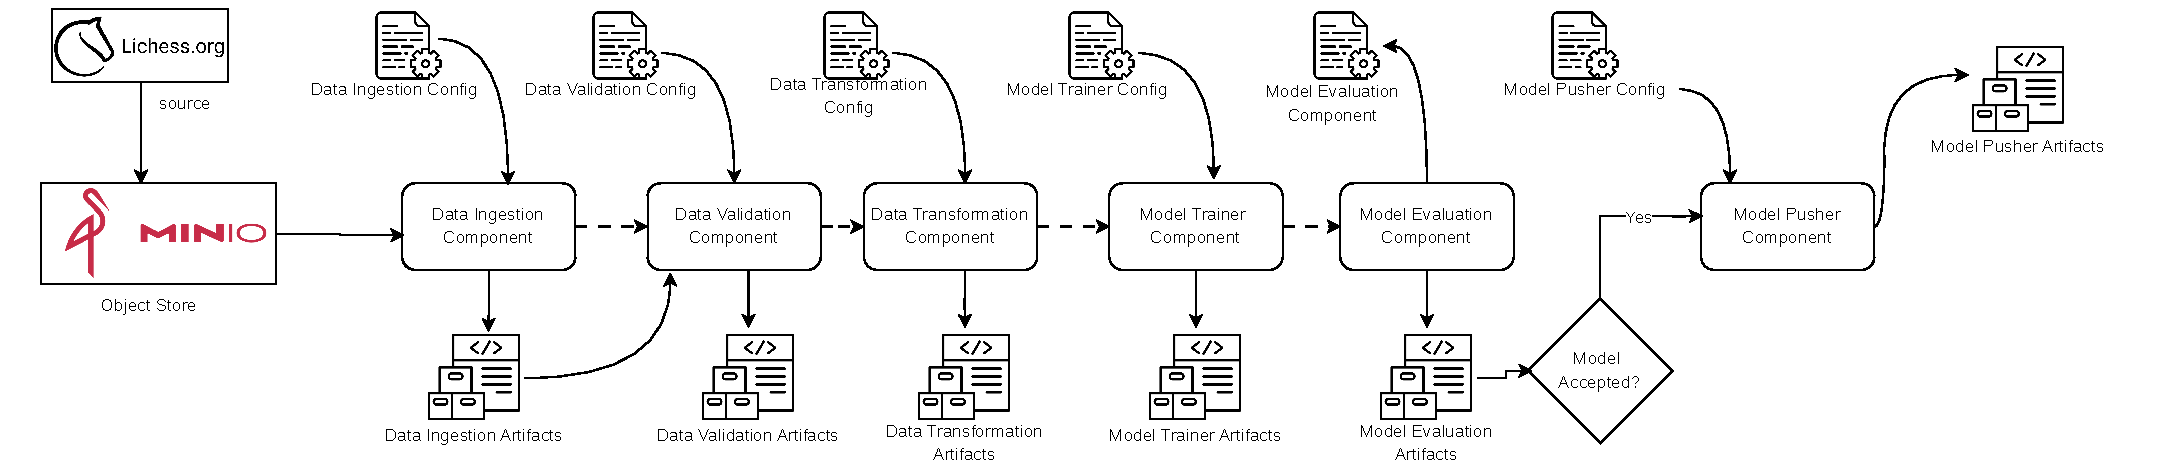
\includegraphics[width=\linewidth,height=0.92\textheight,keepaspectratio]{arch_diag.pdf}
  \caption{End-to-end MLOps pipeline: raw Lichess data lands in MinIO; sequential components (configuration plus prior artefacts $\rightarrow$ processing $\rightarrow$ new artefacts) cover ingestion, validation, transformation, training, and evaluation; a decision gateway permits model push only when evaluation guardrails pass.}
  \label{fig:mlops-pipeline}
\end{figure}

\begin{figure}[htbp]
  \centering
  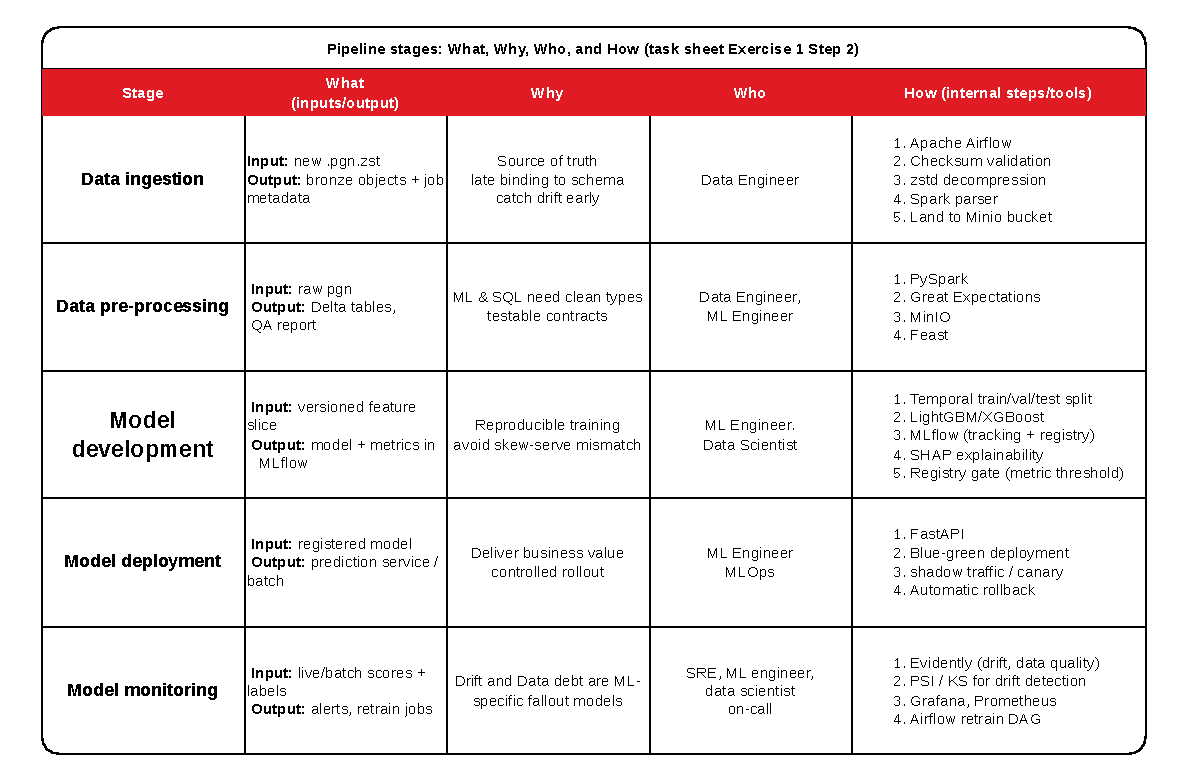
\includegraphics[width=\linewidth,keepaspectratio]{whowhatandhow.pdf}
  \caption{Pipeline stages: what (inputs and outputs), why (rationale), who (accountability), and how (internal steps and tools) for ingestion through monitoring (Exercise~1, Step~2).}
  \label{fig:pipeline-whowhatandhow}
\end{figure}

\Cref{fig:etl-flow} shows Airflow bucket ETL; \cref{fig:mlops-pipeline} shows immutable artefact stages through validation, training, evaluation, and conditional push; \cref{fig:pipeline-whowhatandhow} tabulates what, why, who, and how for each mandated stage.
The sections below elaborate each stage with dedicated diagrams.

\section{Data ingestion}
\label{sec:stage-ingestion}

\begin{figure}[htbp]
  \centering
  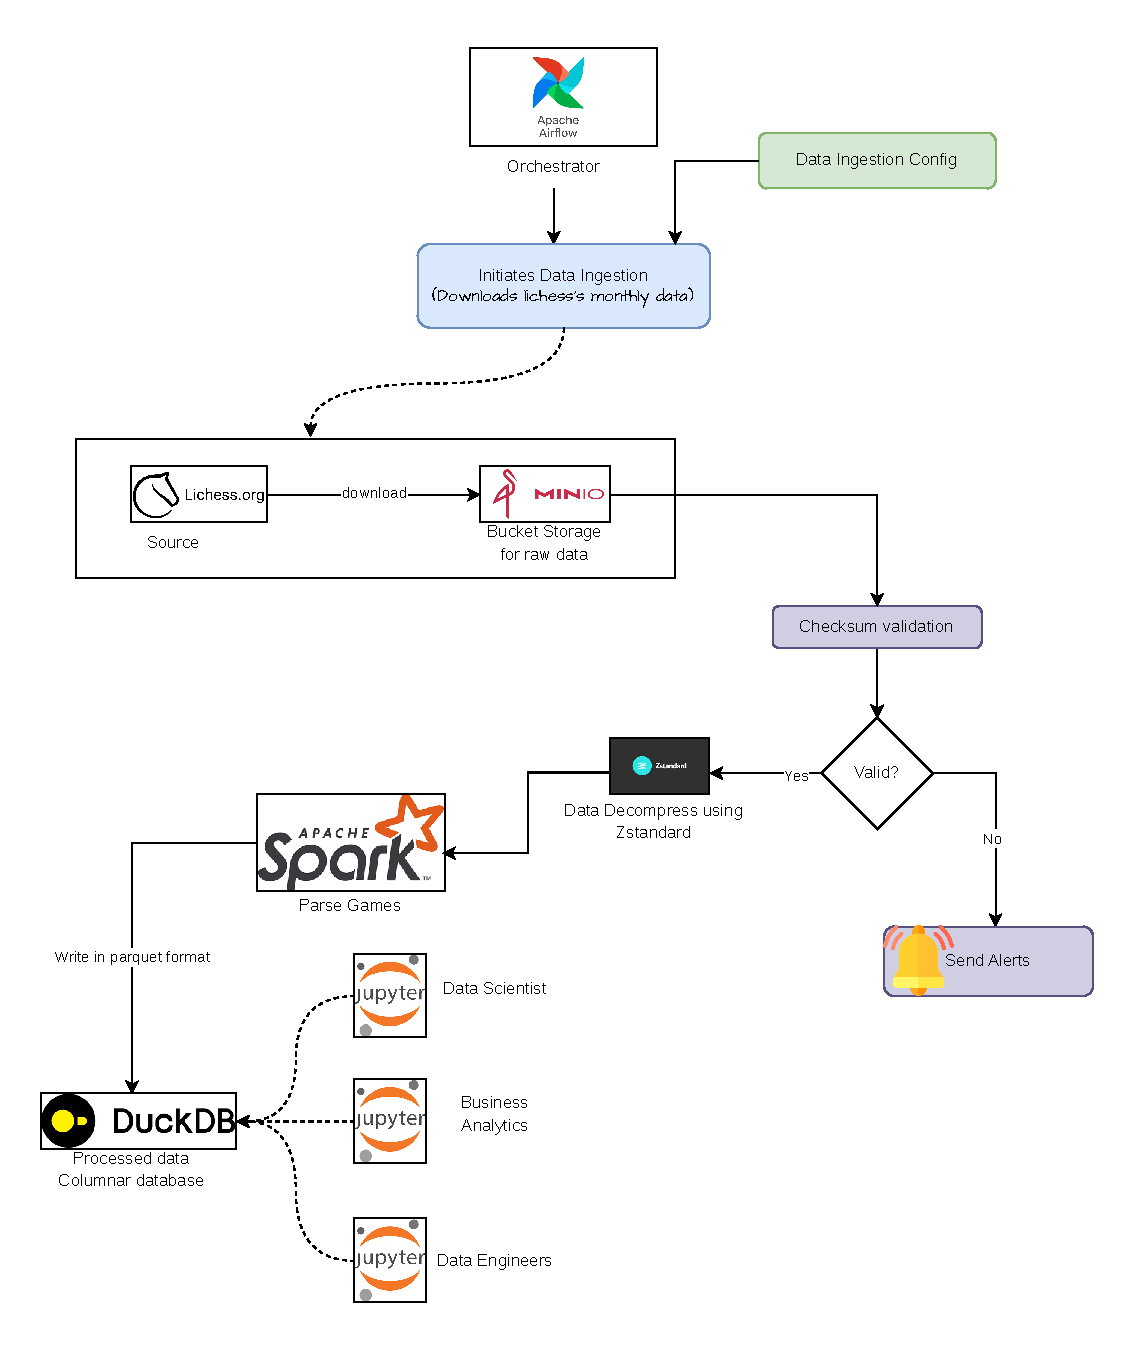
\includegraphics[width=\linewidth,height=0.85\textheight,keepaspectratio]{dataIngestion.pdf}
  \caption{Data ingestion: the orchestrator applies ingestion config, downloads Lichess monthly data to a raw-data bucket, validates checksums, decompresses with Zstandard, parses games, and writes processed Parquet; invalid payloads trigger alerts.}
  \label{fig:data-ingestion}
\end{figure}

Ingestion lands bulk \texttt{.pgn.zst} in MinIO with monthly partitions, checksum contracts, and idempotent keys (\cref{fig:data-ingestion}).
Data engineering owns connectors; governance checks licensing.
Stable landing prevents gaps and duplicates that would break dashboards and labels.

\section{Data pre-processing}
\label{sec:stage-preprocessing}

\begin{figure}[htbp]
  \centering
  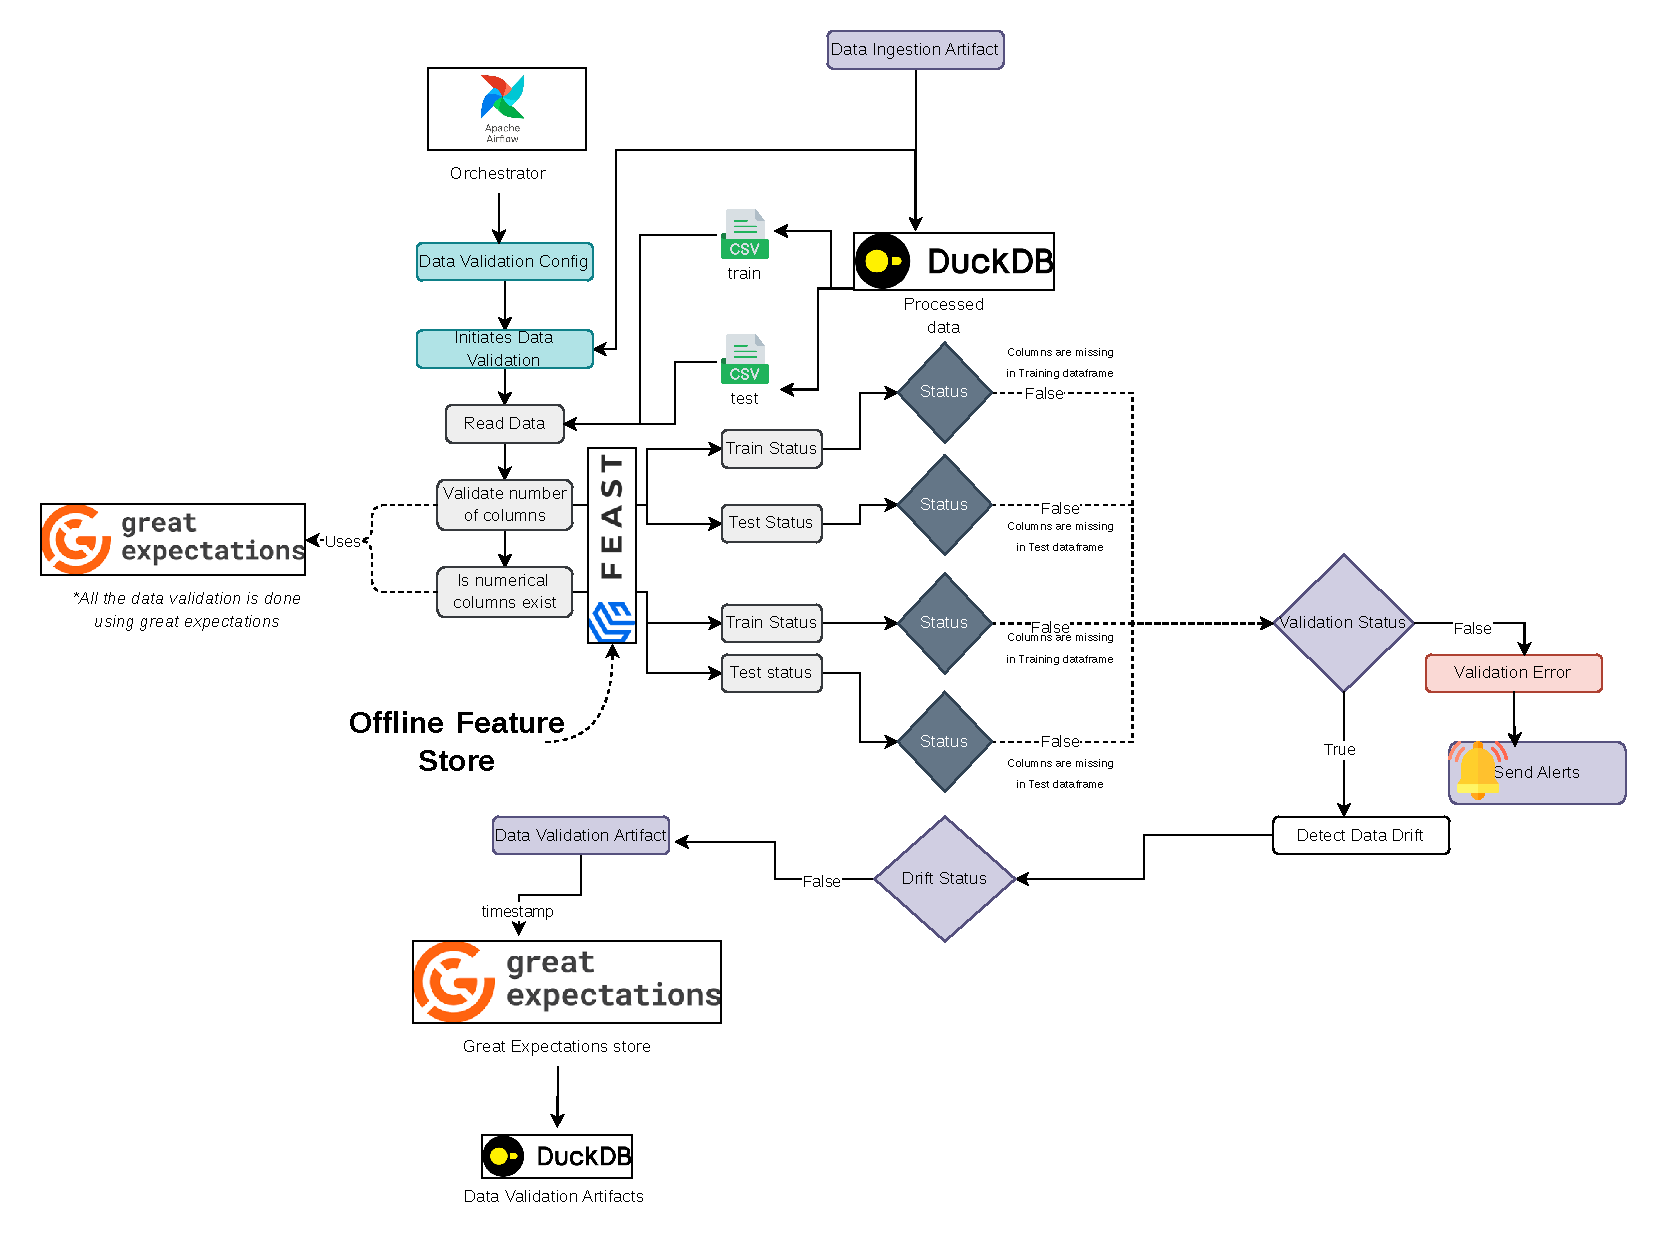
\includegraphics[width=\linewidth,height=0.92\textheight,keepaspectratio]{dataValidation.pdf}
  \caption{Data validation under orchestration: train/test splits are checked for schema completeness and drift; Great Expectations stores validation reports; failures route to alerts and updated artefact keys, while validated processed data feeds an offline feature store.}
  \label{fig:data-validation}
\end{figure}

Validation enforces schema and drift budgets; transformation encodes features, splits without leakage, and serialises preprocessors beside tensors (\cref{fig:data-validation}).
SMEs tune rules; automation blocks downstream on threshold breaches.
Analysts consume silver tables; training reuses the same transforms at inference.

\section{Model development}
\label{sec:stage-model-dev}

\begin{figure}[htbp]
  \centering
  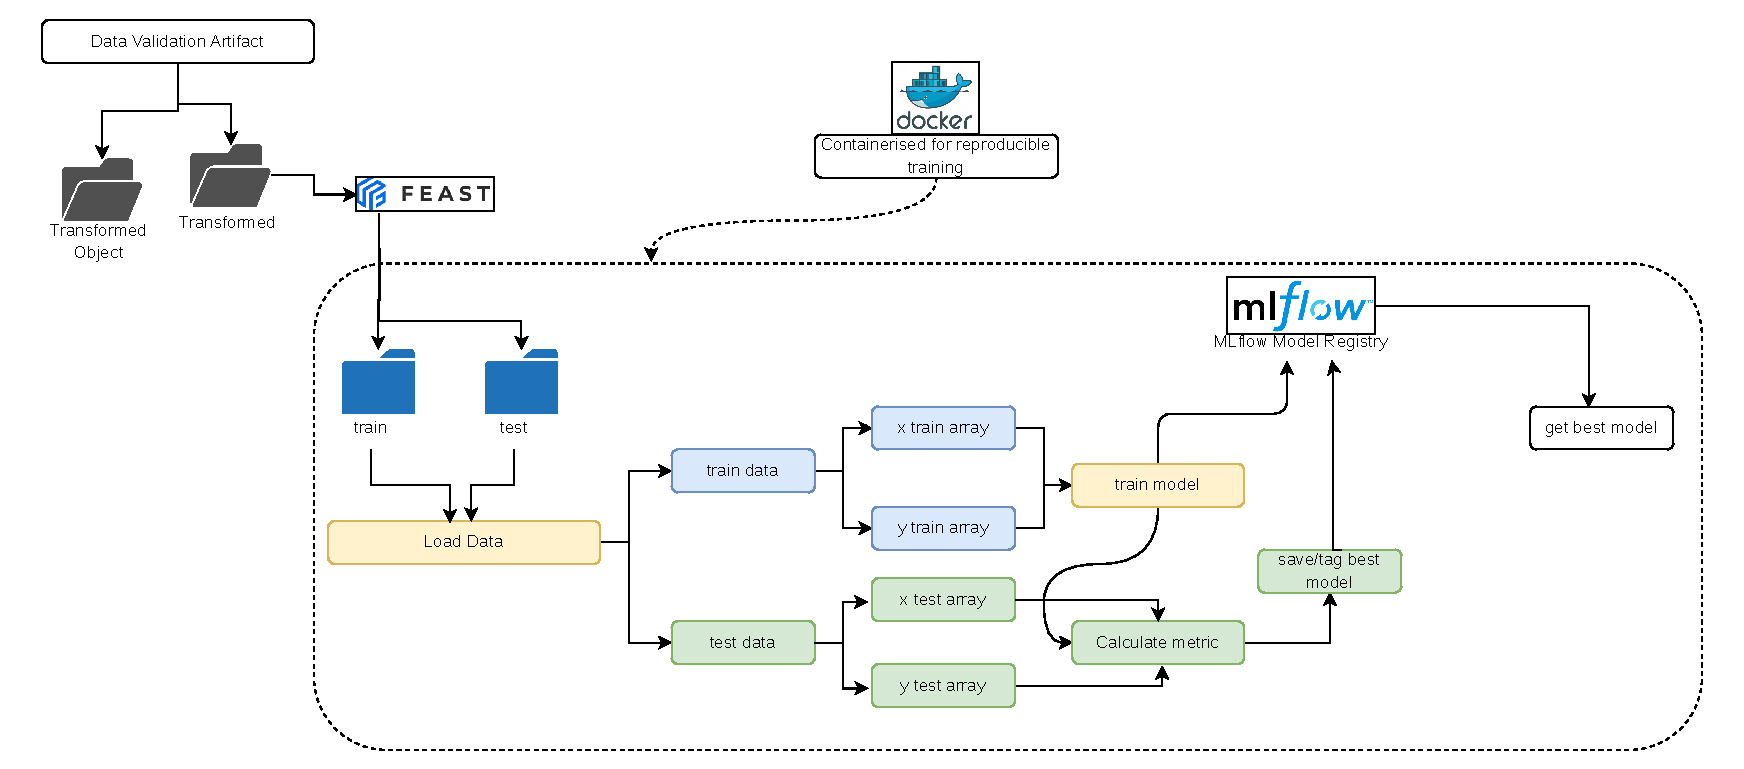
\includegraphics[width=\linewidth,height=0.85\textheight,keepaspectratio]{modelTrainer.pdf}
  \caption{Model training: load train/test arrays from validated artefacts, fit the model, compute metrics, register the best run in MLflow, and retain a containerised, reproducible training environment.}
  \label{fig:model-trainer}
\end{figure}

Training reads transform bundles and logs git, configs, and metrics in MLflow (\cref{fig:model-trainer}).
Research approves hypotheses; engineers run sweeps with sequestered test data until final evaluation exports.

\section{Model deployment}
\label{sec:stage-deployment}

\begin{figure}[htbp]
  \centering
  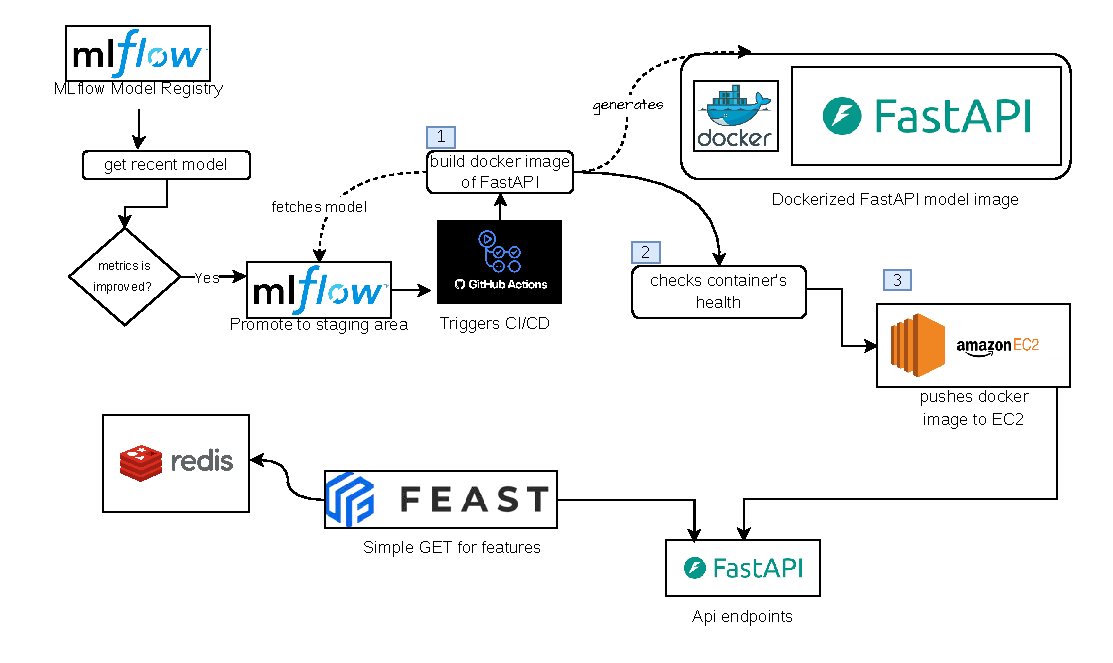
\includegraphics[width=\linewidth,height=0.85\textheight,keepaspectratio]{deployment.pdf}
  \caption{Deployment: promote a recent model from MLflow, build a Dockerised FastAPI image, run health checks, and push to the serving host (e.g.\ EC2); improved metrics can trigger CI/CD to refresh the endpoint.}
  \label{fig:deployment}
\end{figure}

Containers promote only after gates; MLOps owns CI/CD with SecOps image review (\cref{fig:deployment}).
Canary and rollback retag registries; contracts keep serving aligned with preprocessing.

\section{Model monitoring}
\label{sec:stage-monitoring}

\begin{figure}[htbp]
  \centering
  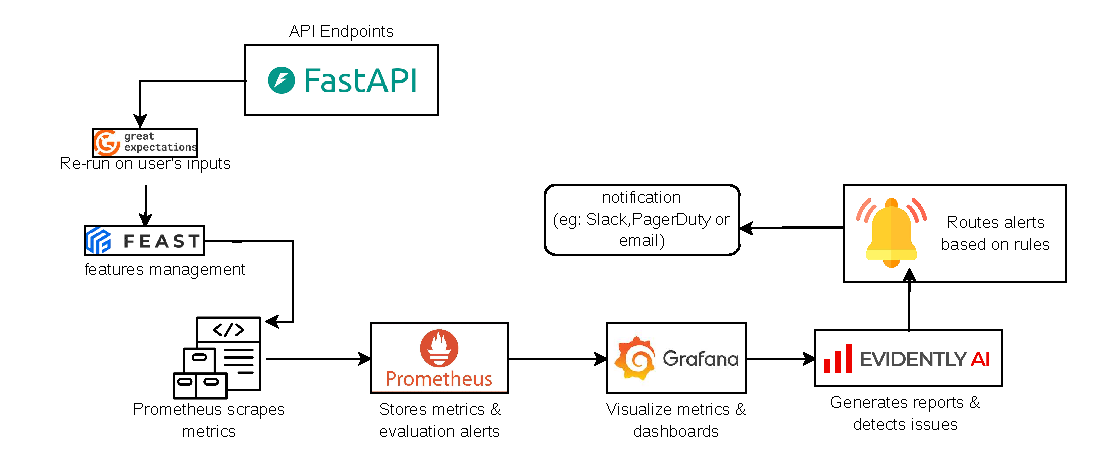
\includegraphics[width=\linewidth,height=0.85\textheight,keepaspectratio]{monitoringObserv.pdf}
  \caption{Monitoring and observability: API metrics scraped by Prometheus, dashboards and automated reports, rule-based routing to Slack/PagerDuty/email, and controlled reruns from user or scheduled inputs.}
  \label{fig:monitoring}
\end{figure}

Production tracks feature drift, latency SLOs, and score error as new months arrive (\cref{fig:monitoring}).
MLOps triages alerts; retrains stay lineage-linked to ingestion batches.

\section{Iterative refinement narrative}
\label{sec:iteration-pipeline}

We replaced an early sketch with~\cref{fig:mlops-pipeline} for validation loops and RACI~\cref{tab:pipeline-raci-lite}.

\begin{table}[htbp]
  \centering
  \caption{Pipeline stage accountability matrix (illustrative).}
  \label{tab:pipeline-raci-lite}
  \footnotesize
  \setlength{\tabcolsep}{4pt}
  \renewcommand{\arraystretch}{1.1}
  \begin{tabular}{@{}>{\raggedright\arraybackslash}p{0.31\linewidth} >{\centering\arraybackslash}p{0.115\linewidth}>{\centering\arraybackslash}p{0.115\linewidth}>{\centering\arraybackslash}p{0.115\linewidth}>{\centering\arraybackslash}p{0.115\linewidth}@{}}
    \toprule
    Pipeline stage & R & A & C & I\\
    \midrule
    Data ingestion             & DE & Head of data & Stewardship & Analysts\\
    Data pre-processing        & DE / MLE & MLOps lead & Domain SMEs & Governance\\
    Model development          & MLE & Research lead & SMEs & Analysts\\
    Model deployment           & MLOps & Prod owner & SecOps & Analysts\\
    Model monitoring           & MLOps & Prod owner & MLE \& DE & Stewardship\\
    \bottomrule
  \end{tabular}
\end{table}

\textbf{Legend:}
\textit{R}esponsible performs the hands-on work,
\textit{A}ccountable approves outcomes,
\textit{C}onsulted offers domain expertise,
\textit{I}nformed stays aware of timelines.

\chapter{Data Storage Plan}
\label{ch:storage-planning}
This chapter focuses on the data decisions taken while designing the MLOps pipeline. Further this section also discusses about the physical and logical structure of the dataset showcasing how the current design decisions helps in making the optimal for data analytics and downstream meaching learning tasks too.  

% Chapters~\cref{ch:candidate-datasets}--\cref{ch:pipeline-planning} fix corpus plus DAG scope; landing and joins only~\cite{lichess_open_database}.

\section{Data Source}
\label{sec:storage-source}
The data is from Lichess platform which is an open source alternative version of chess.com for playing chess online. Lichess publishes its entire games from database for public use at \url{database.lichess.org}. It is a bulk file which can be downloaded over HTTPS. Each month a single compressed file is published alongside a SHA256 checksum for validation. This project downloads those files, verifies it, and lands it in the object store named MinIO. 

\subsection{Physical Storage}
\label{sec:storage-provenance}
The raw file downloaded from Lichess which is downloaded and stored in object storage is a compressed PGN file using Zstandard. Zstandard (zstd) was chosen by Lichess because of its balance for compression ration and decompression speed. Once decompressed, the plain-text PGN is roughly five times larger. A typical month goes from ~20 GB to ~100 GB. The raw file remains in the lake as a single immutable object with no transformation is done at this stage.

% \texttt{database.lichess.org} publishes monthly \texttt{.pgn.zst} shards plus checksum pairs; verified copies sit in MinIO with inventory in~\cref{app:lichess-open-database}~\cite{lichess_open_database}.

\subsection{Logical Storage}
\label{sec:logical-storage}
The PGN format is semi-structured file format for storage chess games with metadata. There is no enforeced schema but the structure repeats reliably. Every game is a block of following components:

\begin{enumerate}
    \item A set of headers
    \item An empty line in between
    \item The move list in Standard Algebraic Notation. Some games also contains evaluation from stockfish chess engine.
\end{enumerate}



Logically we can think of the dataset as two nested entities.
\begin{enumerate}
 \item \textbf{Game:} Fixed attributes (date, players, result, opening, etc.).
 \item \textbf{Move:} An ordered list of half-moves, each carrying a move number, SAN notation, UCI coordinates, evaluation, and clock remaining. 
\end{enumerate}

The cardinality is one game to zero-or-many moves.

\section{Ingested Data Storage}
\label{ingested_data_storage}
After extraction and loading, the raw \texttt{.zst} object is transformed into a set of Parquet tables arranged in a star schema. I follow an ELT pattern: the compressed file lands unchanged in MinIO first (load), then Apache Spark reads from object storage to parse and shape the data (transform), and the curated tables are written to MinIO as Parquet and loaded into DuckDB for analytics.


\subsection{Why Parquet?}
\begin{itemize}
    \item Fast aggregations (scans only the columns needed).
    \item High compression (columns hold similar data).
    \item Predicate push-down with Spark/DuckDB (partition pruning on year/month).
\end{itemize}

\subsection{Why MinIO?}
It keeps compute and storage separate, allows direct S3-compatible reads from Spark, DuckDB, and Feast, and the raw bucket gives a permanent, immutable copy for reprocessing.

\subsection{Logical structure (Star Schema)}
The processed data is modelled as a star schema centred on \texttt{fact\_games}. The design is shown in \cref{fig:dataset-one-logical-erd} as a crow-foot ERD.

\begin{figure}[htbp]
  \centering
  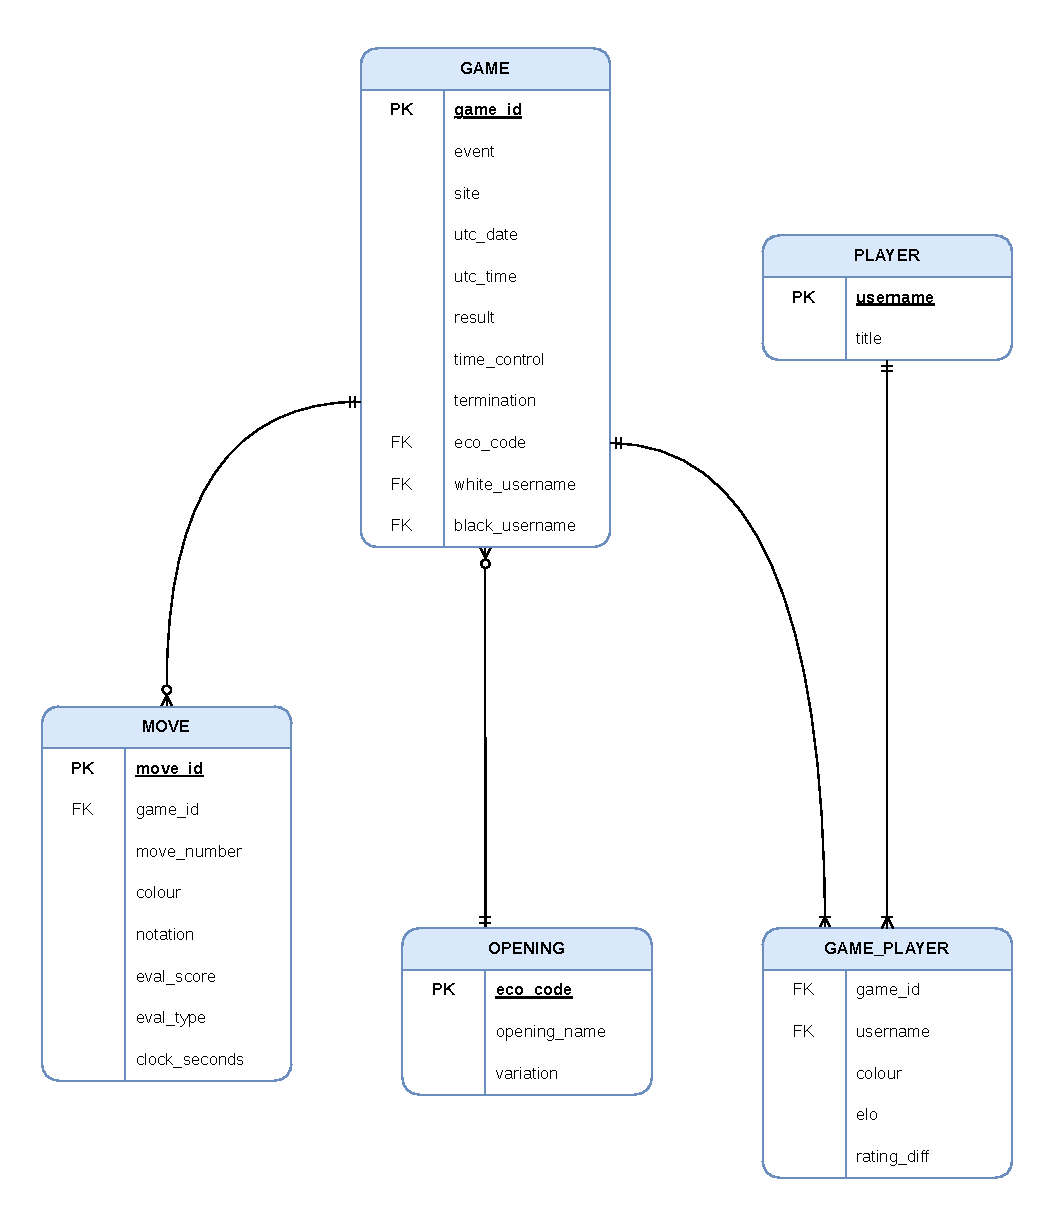
\includegraphics[width=0.95\linewidth,height=0.85\textheight,keepaspectratio]{erd}
  \caption{Star schema for processed Lichess data: a central fact table of games with dimensions for players, openings, and dates.}
  \label{fig:dataset-one-logical-erd}
\end{figure}



\subsection{Justification for the star schema}
The star schema was chosen because it directly supports the two main consumer groups in the pipeline:


\begin{table}[htbp]
    \centering
    \renewcommand{\arraystretch}{1.5}
    \begin{tabular}{|p{0.3\textwidth}|p{0.65\textwidth}|}
        \hline
        \textbf{Need} & \textbf{How the star schema meets it} \\ \hline
        ML feature engineering (Feast) & Feast works with entity keys; the fact table and dimensions can be mapped to Feast FeatureViews with simple joins on player, opening, or date keys. Point-in-time joins are straightforward. \\ \hline
        Analyst / Data Scientist notebooks & A single join from the fact table to a dimension is enough for most queries; no complex multi-table logic. \\ \hline
        Storage efficiency & Player attributes (username, title) are stored once, not repeated per game. Parquet columnar compression reduces the footprint further. \\ \hline
        Incremental monthly loads & Partitioning on year/month means new months are appended; dimensions are updated with a merge without rewriting the whole fact table. \\ \hline
        Data quality checks & Each table can have a dedicated Great Expectations suite (e.g., null checks on fact columns, uniqueness on dimension keys). \\ \hline
    \end{tabular}
\end{table}

\section{Benefits, drawbacks and Mitigation of the star schema}
The star schema model is straightforward to communicate to both engineers and data scientists because breaking the dataset into games, players, openings, and dates maps naturally to the chess domain. By using this approach, we avoid the massive data duplication that typically plagues a single, wide table. This structure also perfectly complements the write-once, read-many nature of historical chess data. While queries requiring multiple dimensions do need joins, the dimensions are relatively small, and engines like DuckDB or Spark manage these columnar joins quite efficiently. We accepted a minor bit of redundancy, such as storing the \texttt{last\_known\_elo} directly in the \texttt{dim\_player} table instead of constantly recalculating it from the fact table, simply because it makes looking up current ratings significantly faster. Finally, although evolving the schema—like adding a brand new dimension—demands careful coordination, using Parquet makes this manageable by supporting schema merging and allowing new dimensions to be introduced independently over time.

\section{Alternative structure}
\begin{table}[htp!]
    \centering
    \begin{tabular}{|p{3cm}|p{3.5cm}|p{4.5cm}|p{3.5cm}|}
        \hline
        \textbf{Approach} & \textbf{Upside} & \textbf{Downside \& Mitigation} & \textbf{Why not chosen} \\ \hline
        One Big Table & Zero joins, simple CSV & Huge duplication, brittle schema, breaks temporal correctness & Duplication and temporal fidelity risk too high \\ \hline
        Star Schema (chosen) & Familiar, fits Feast, good compression, incremental & Joins needed; mitigated by columnar scans and small dimensions & --- \\ \hline
        Snowflake & Even less redundancy in dimensions & Extra joins for minimal gain (shallow ECO hierarchy) & Complexity doesn’t pay off \\ \hline
        3NF relational & Clean updates, no anomalies & Many‑table joins hurt read speed at scale & Append‑heavy workload; read performance more important \\ \hline
        Medallion layers & Clear quality gates & Overlaps with raw/processed bucket split & Redundant; our raw bucket already provides the “bronze” layer \\ \hline
    \end{tabular}
\end{table}


\section{Extraction, Loading, and Transformation (ELT)}
I follow an ELT pattern because the heavy transformation happens after the data lands in the object store MinIO.

\begin{figure}[htbp]
  \centering
  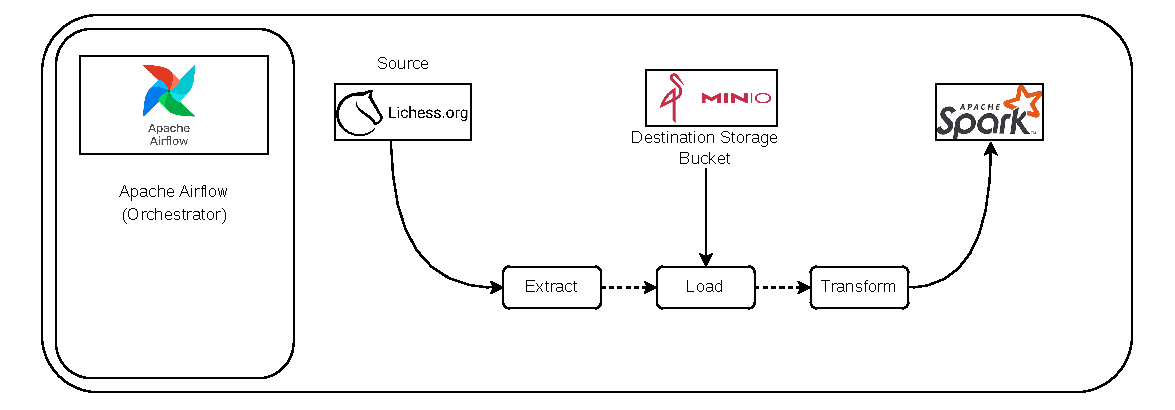
\includegraphics[width=\linewidth,height=0.55\textheight,keepaspectratio]{elt.pdf}
  \caption{ELT pattern with object storage.}
  \label{fig:elt-flow}
\end{figure}



\subsection{Extract}
An Airflow DAG fetches each monthly \texttt{.pgn.zst} file from Lichess over HTTPS and checks it against the published SHA256 checksum. A mismatch fails the task and triggers an alert.

\subsection{Load}
The verified file lands in MinIO at \texttt{s3://lichess-raw/pgn/...} without decompression or parsing. It stays there as an immutable archive until Spark reads it.

\subsection{Transform}
PySpark streams the \texttt{.zst} object from MinIO, decompresses it in-flight, and parses games with a python-chess UDF. Headers and derived fields (e.g.\ move count) go to \texttt{fact\_games}; half-moves, engine evaluations, and clock times optionally go to \texttt{fact\_moves}. Distinct players, openings, and dates are merged into \texttt{dim\_player}, \texttt{dim\_opening}, and \texttt{dim\_date}. Curated tables are written to \texttt{s3://lichess-processed/} as Parquet, with fact tables partitioned by year and month.

\subsection{Validation}
Great Expectations runs a checkpoint on each new partition (schema, null rates, value bounds). Partitions that pass are released to Feast and analyst notebooks.


\chapter{Reflective discussion}
\label{ch:reflection}

\begin{figure}[htbp]
  \centering
  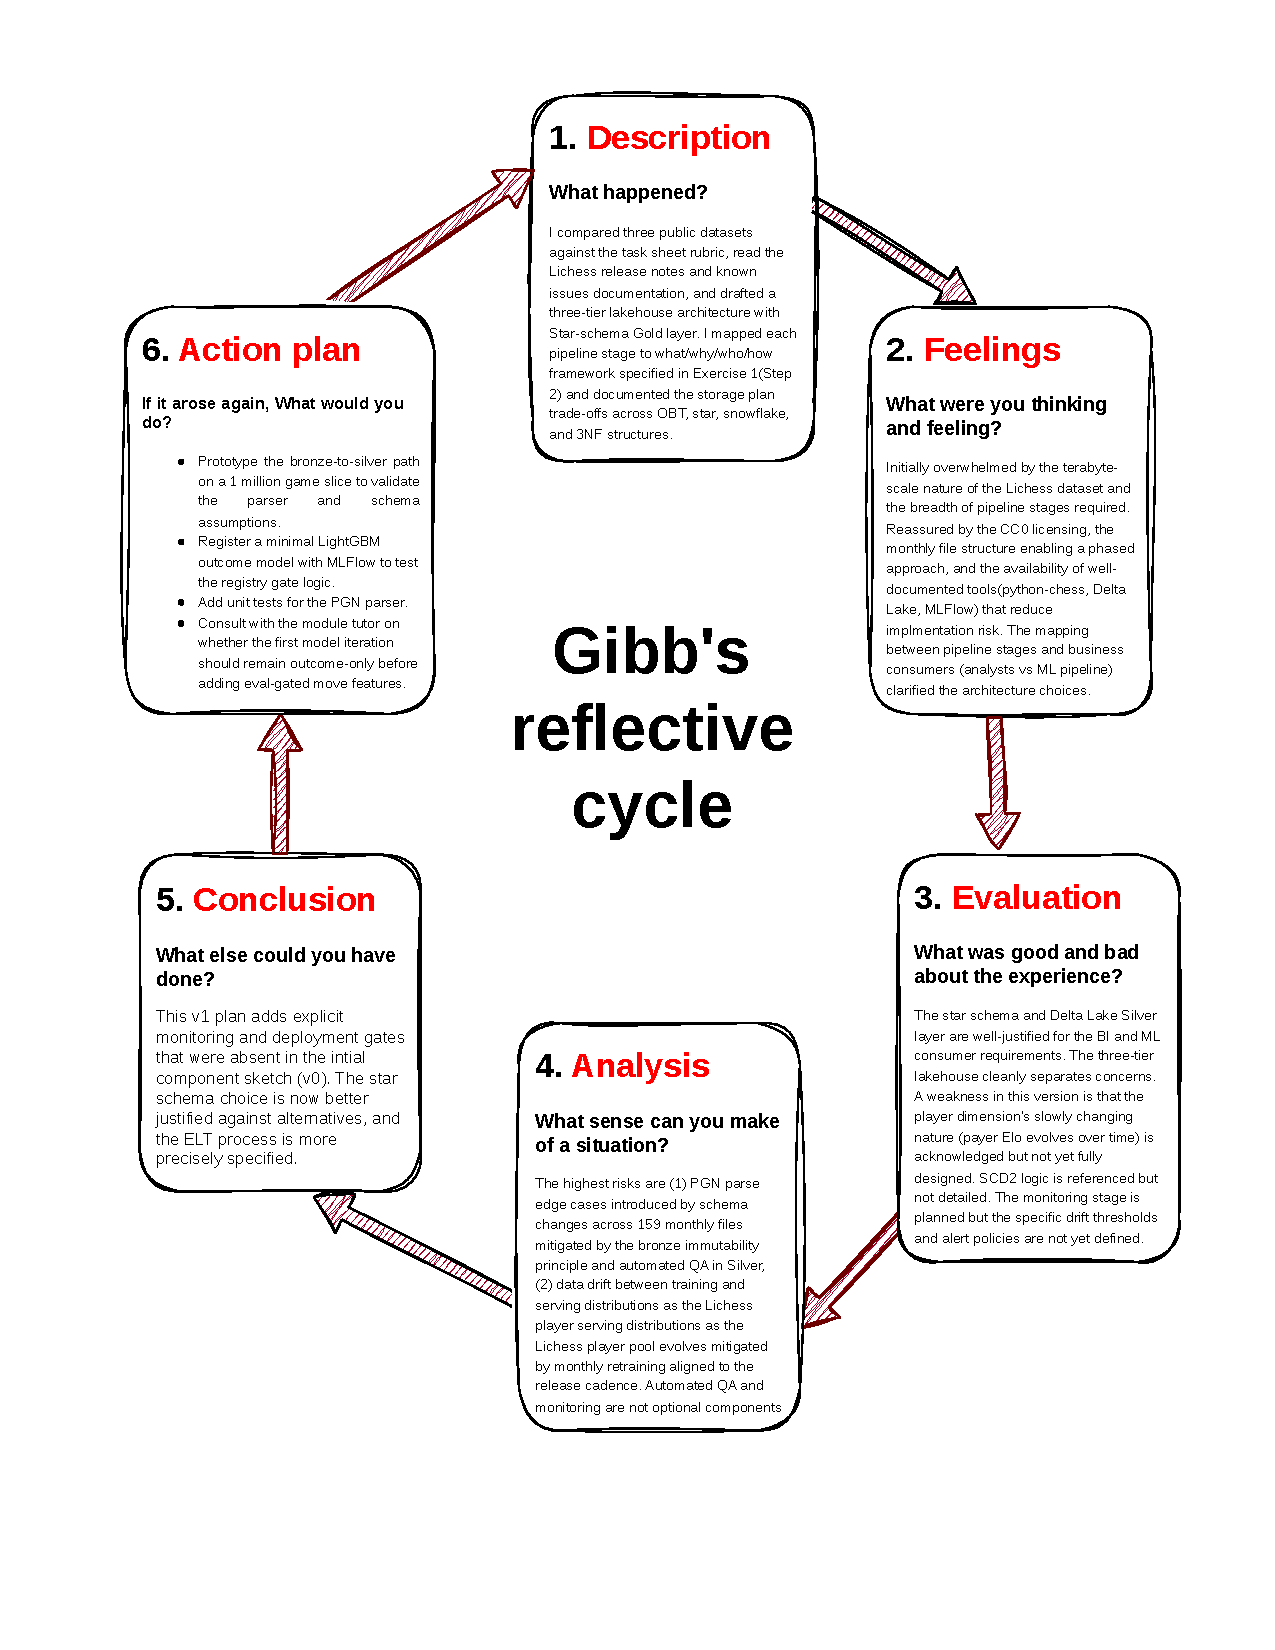
\includegraphics[width=0.95\linewidth,height=0.65\textheight,keepaspectratio]{reflection}
  \caption[Gibb's reflective cycle for iterative MLOps planning.]{\textit{Gibb's reflective cycle} applied to iterative planning for the Lichess MLOps design.}
  \label{fig:reflection-iterations}
\end{figure}

This planning pass showed how sharply storage choices diverge from pipeline choreography once volume grows:~\cref{fig:mlops-pipeline} sequences Airflow stages, whereas~\cref{ch:storage-planning} had to freeze Parquet partitions and surrogate keys before analysts could safely join~\cref{fig:storage-star-erd}.
The star-versus-wide-table tension was formative---duplicated player columns tempted me until schema churn on hundreds of millions of rows made normalised dimensions unavoidable.
Iteratively, laptop CSV pilots collapsed under monthly Lichess drops, forcing the lake ELT story aligned with~\cref{fig:etl-flow} and immutable MinIO prefixes~\cite{lichess_open_database}.
\Cref{fig:reflection-iterations} reminds me to record each Gibbs stage when diagrams change so future retrains cite exact artefact vintages.
If I repeated the task, I would co-author Great Expectations suites beside the ingestion DAG definition, checkpoint partition conventions in git with orchestration tweaks, and run prose word-limit checks beside \texttt{latexmk}.


\appendix

\chapter{Supplementary material}
\label{app:supplementary}

Use this appendix for oversized diagrams or repeat tables referenced in the body.
Keeping the narrative readable in the main chapters while placing detailed artefacts here is conventional for coursework and technical reports alike.

\printbibliography[heading=bibintoc]

\end{document}
